\documentclass[11pt,a4paper]{article}
    \usepackage[margin=2.5cm]{geometry}
    \usepackage{enumitem}
    \usepackage{hyperref}
    \usepackage{tikz}
    \usetikzlibrary{arrows.meta,positioning,shapes.geometric}
    \title{Machine Learning Teaching Tools}
\author{Jordi Vill\`a-Freixa \texttt{<jordi.villa@uvic.cat>}}
    \date{\today}

    \tikzset{
      methodbox/.style={
        rounded corners=6pt,
        draw=blue!50!black,
        line width=0.9pt,
        fill=blue!6,
        minimum width=13cm,
        text width=11.8cm,
        align=left,
        inner sep=8pt
      }
    }

    \begin{document}
    \maketitle

    \section*{Scope}
    This folder contains compact teaching notebooks for dimensionality reduction and supervised latent-variable models. The emphasis is on interpretable workflows rather than production ML pipelines.

    \section*{Material in this folder}
    \begin{itemize}[leftmargin=*]
\item \texttt{BasicPLS.ipynb}
\item \texttt{PCA\_PLS.ipynb}
    \end{itemize}

    \section*{Method summary}
    \begin{itemize}[leftmargin=*]
\item \textbf{Principal component analysis}. The PCA material projects multivariate data onto orthogonal directions that maximize explained variance.
\item \textbf{Partial least squares regression}. The PLS notebooks relate predictors and responses through latent variables that maximize covariance between both blocks.
\item \textbf{Score and loading interpretation}. The notebooks use scores, loadings, and explained variance to interpret structure in the data.
    \end{itemize}

    \section*{Method scheme}
    Figure~\ref{fig:summary} is drawn directly in LaTeX with TikZ. It is a compact conceptual map of the main workflows discussed in this folder.

    \begin{figure}[ht]
    \centering
    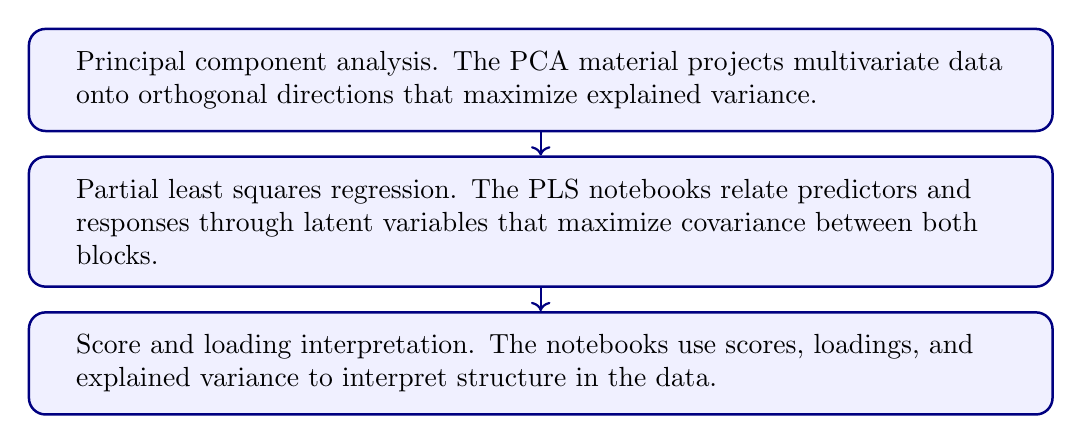
\begin{tikzpicture}[x=1cm,y=1cm]
    \node[methodbox] (m0) at (0,0.0) {Principal component analysis. The PCA material projects multivariate data onto orthogonal directions that maximize explained variance.};
    \node[methodbox] (m1) at (0,-1.8) {Partial least squares regression. The PLS notebooks relate predictors and responses through latent variables that maximize covariance between both blocks.};
    \node[methodbox] (m2) at (0,-3.6) {Score and loading interpretation. The notebooks use scores, loadings, and explained variance to interpret structure in the data.};
    \draw[->, thick, color=blue!50!black] (m0.south) -- (m1.north);
    \draw[->, thick, color=blue!50!black] (m1.south) -- (m2.north);
    \end{tikzpicture}
    \caption{Conceptual scheme for the methods in the MLtools folder.}
    \label{fig:summary}
    \end{figure}

    
\bibliographystyle{plain}
\bibliography{../references}

\section*{Disclaimer}
These documents were generated with the assistance of ChatGPT 5.4. The material has been reviewed by the author before inclusion in this repository, but it is not free from possible errors.

\end{document}